\documentclass[
fontsize=12pt,					% Schriftgröße
paper=a4,						% Papierformat
twoside=true, 					% einseitiges (false) oder zweiseitiges (true) Dokument
listof=totoc, 					% Tabellen- und Abbildungsverzeichnis ins Inhaltsverzeichnis
bibliography=totoc,				% Literaturverzeichnis ins Inhaltsverzeichnis aufnehmen
titlepage, 						% Titlepage-Umgebung statt \maketitle
headsepline, 					% horizontale Linie unter Kolumnentitel
%abstracton,					% Überschrift beim Abstract einschalten, Abstract muss dazu in {abstract}-Umgebung stehen
DIV=12,							% Satzspiegeleinstellung, 12 ist Standar bei KOMA
BCOR=6mm,						% Bindekorrektur, die den Seitenspiegel um 3mm nach rechts verschiebt,
cleardoublepage=empty,			% Stil einer leeren eingefügten Seite bei Kapitelwechsel
parskip,							% Absatzabstand bei Absatzwechsel einfügen
ngerman
]{scrartcl}

\usepackage[setspace=false]{scrhack}
\usepackage[utf8]{inputenc} 	% ermöglicht die direkte Eingabe von Umlauten
\usepackage[T1]{fontenc} 		% Ausgabe aller zeichen in einer T1-Codierung (wichtig für die Ausgabe von Umlauten!)
\usepackage{babel} 	% deutsche Trennungsregeln und Übersetzung der festcodierten Überschriften
\renewcaptionname{ngerman}{\contentsname}{Inhaltsverzeichnis}
\renewcaptionname{ngerman}{\bibname}{Literaturverzeichnis}
\setlength{\parindent}{0ex} 	% bei neuem Abschnitt nicht einrücken

\newcommand{\lowrule}{%
	\leavevmode \kern.06em\vbox{\hrule width.5em}}

\usepackage{siunitx}			% Vereinfachte Eingabe von Einheiten in Formeln
\sisetup{
	number-unit-product = \;,
	inter-unit-product = \:,
	exponent-product = \cdot,
	output-decimal-marker = {,}
}

\usepackage{graphicx}  			% Einbinden von Grafiken erlauben
\usepackage[format=hang,		% Formatierungen von Unter- / Überschriften
font=normal,
labelfont=bf,
justification=RaggedRight,
singlelinecheck=true,
aboveskip=1mm
]{caption}

\usepackage[backend=biber, %% Hilfsprogramm "biber" beim Compilieren nutzen (statt "biblatex" oder "bibtex")
style=numeric, %% Zitierstil (siehe Dokumentation)
natbib=true, %% Bereitstellen von natbib-kompatiblen Zitierkommandos
hyperref=true, %% hyperref-Paket verwenden, um Links zu erstellen
]{biblatex}

\usepackage{pdfpages}

\usepackage{enumitem}			% Erlaubt Änderung der Nummerierung in der Umgebung enumerate

\usepackage{amsmath}			% Ergänzungen für Formeln
\usepackage{textcomp} 			% zum Einsatz von Eurozeichen u. a. Symbolen
\usepackage{eurosym}			% bessere Darstellung Euro-Symbol mit \euro

\usepackage[					% Einstellunge Paket hyperref
hyperfootnotes=false,			% im pfd-Output Fußnoten nicht verlinken
hidelinks						% Entfernen von farbigen Umrandungen der Links
]{hyperref}

\usepackage[					% Einstellungen für Fußnoten
bottom,							% Ausrichtung unten
multiple,						% Trennung durch Seperator bei mehreren Fußnoten
hang,
marginal
]{footmisc}

\usepackage{calc}				% Paket zum Berechnen von Längen z.B. 0.8\linewidth

\usepackage{xcolor} 			% einfache Verwendung von Farben in nahezu allen Farbmodellen

\usepackage{listings}			% Darstellung von Quellcode mit den Umgebungen {lstlisting}, \lstinline und \lstinputlisting
\lstset{literate=				% Damit können Umlaute innerhalb Listings geschrieben werden
	{Ö}{{\"O}}1
	{Ä}{{\"A}}1
	{Ü}{{\"U}}1
	{ß}{{\ss}}1
	{ü}{{\"u}}1
	{ä}{{\"a}}1
	{ö}{{\"o}}1
}
\definecolor{mygreen}{rgb}{0,0.6,0}
\definecolor{mygray}{rgb}{0.5,0.5,0.5}
\definecolor{mymauve}{rgb}{0.58,0,0.82}
\lstset{ %
	backgroundcolor=\color{white},   % choose the background color; you must add \usepackage{color} or \usepackage{xcolor}; should come as last argument
	basicstyle=\footnotesize,        % the size of the fonts that are used for the code
	breakatwhitespace=false,         % sets if automatic breaks should only happen at whitespace
	breaklines=true,                 % sets automatic line breaking
	captionpos=t,                    % sets the caption-position to (b) bottom or (t) top
	commentstyle=\color{mygreen},    % comment style
	deletekeywords={...},            % if you want to delete keywords from the given language
	escapeinside={\%*}{*)},          % if you want to add LaTeX within your code
	escapeinside={(*@}{@*)},
	extendedchars=true,              % lets you use non-ASCII characters; for 8-bits encodings only, does not work with UTF-8
	frame=none,	                   	% "single" adds a frame around the code; "none"
	keepspaces=true,                 % keeps spaces in text, useful for keeping indentation of code (possibly needs columns=flexible)
	keywordstyle=\color{blue},       % keyword style
	language=[LaTeX]TeX,             % the language of the code
	morekeywords={*,nomenclature},   % if you want to add more keywords to the set
	numbers=left,                    % where to put the line-numbers; possible values are (none, left, right)
	numbersep=5pt,                   % how far the line-numbers are from the code
	numberstyle=\tiny\color{mygray}, % the style that is used for the line-numbers
	rulecolor=\color{black},         % if not set, the frame-color may be changed on line-breaks within not-black text (e.g. comments (green here))
	showspaces=false,                % show spaces everywhere adding particular underscores; it overrides 'showstringspaces'
	showstringspaces=false,          % underline spaces within strings only
	showtabs=false,                  % show tabs within strings adding particular underscores
	stepnumber=1,                    % the step between two line-numbers. If it's 1, each line will be numbered
	stringstyle=\color{mymauve},     % string literal style
	tabsize=2,	                   % sets default tabsize to 2 spaces
	title=\lstname                   % show the filename of files included with \lstinputlisting; also try caption instead of title
}

% Folgende Zeilen definieren Abkürzungen, um Befehle schneller eingeben zu können
\newcommand{\ua}{\mbox{u.\,a.\ }}
\newcommand{\zB}{\mbox{z.\,B.\ }}
\newcommand{\bs}{$\backslash$}
\newcommand*\diff{\mathop{}\!\mathrm{d}}	% Differentialzeichen
\newcommand*\Diff[1]{\mathop{}\!\mathrm{d^#1}} % Differentialzeichen höherer Ableitung
\newcommand*\jj{\mathop{}\!\mathrm{j}}	% Komplexe Zahl j

% Folgende Zeilen weden benötigt, um Tikz und PGF-Plot-Grafiken einzubinden
\usepackage{pgfplots}
\usepackage{pgfplotstable}
\pgfplotsset{compat=newest,width=0.6\linewidth}
\usepgfplotslibrary{smithchart}
\usepackage{tikz}						% Tikz sollte nach Listings Pakete geladen werden.
\usetikzlibrary{arrows}

\hyphenation{Schrift-ar-ten}

\BeforeClosingMainAux{% siehe KOMA-Script-Anleitung
	\addcontentsline{toc}{chapter}{\indexname}\stepcounter{page}
}

%opening
\title{DeepLearning}
\author{Tim Lucas Halt}

\begin{document}

\maketitle

\begin{abstract}

Sehr kurz

\end{abstract}

\section{Methodik}

Ziel 

Mein Ziel war in einen der drei vorlesungsbegleitende Benchmarks zu führen und die Anstrengungen vorerst auf dieses Ziel zu legen.
Dafür habe ich mich in der ersten Woche in alle drei Richtungen, maximale Genauigkeit, minimale Labels und minimale Parameter probiert.
Zielerreicht wurde mit dem Netzt welches in \autoref{sec:basis} vorgestellt wurde. Eine kombination von verschiedensten quellen zusammengedrafen und mit etwas glück auf 99,47 \% gebracht
Die weitere Verbesserung wollte ich vor allem automatisieren.
Dafür habe ich Kostenlose Grafikkarten von Kaggle (30 Stunden die Woche) und Colab (12 Stunden am Tag) genutzt. 
Im ersten Schritt wollte ich die Wahl der Hyperparemter meines optimieren. dafür habe ich verschiedene Kombinationen mit weights \& biases sweepen und tracken lassen

\section{Basis -  }
\label{sec:basis}

Das Ausgangsnetz, von dem die Betrachtungen ausgehen ist in \autoref{basis} dargestellt. Es hat etwa 62-tausend Parameter. Kompiliert mit dem Adam Optimizer, einer Learning-Rate von 0.003 und einem Training mit dem vollständigen Trainingsdatensatz (60000 Label) bei einer Batch-Size von 512 über 100 Epochen erreichte es 99,47\% Genauigkeit.

\begin{lstlisting}[language=Python, caption=Python-Code, label=basis]
	InputLayer(input_shape=(28,28,1)),
	Conv2D(filter=28, kernel_size=5, padding='same', activation='relu'),
	MaxPooling2D(2,2),
	Conv2D(filter=16, kernel_size=5, padding='same', activation='relu'),
	MaxPooling2D(2,2),
	layers.Dropout(0.2),
	layers.Flatten(),
	layers.Dropout(0.2),
	layers.Dense(64, kernel_regularizer = tf.keras.regularizers.l2(0.07), activation = 'relu'),
	GaussianNoise(0.1),
	Dense(10, activation='softmax')
\end{lstlisting}

\section{Weights and Biases}

Um den Einfluss der Hyperparameter teilautomatisiert zu testen, wird die Sweep-Funktion von Weights \& Biases verwendet (\textcolor{red}{https://docs.wandb.ai/guides/sweeps}. Dabei werden die Hyperparameter aus einem vorgegebenen Raster gewählt, ein Training durchgeführt und die Ergebnisse dokumentiert. Als Methode ist \emph{bayes}, die Bayes'sche Optimierung, zur Maximierung der val\_acc gewählt.

\subsection{Dimensionierung der Filter- und Neuronen-Anzahl}

\begin{figure}
	\centering
	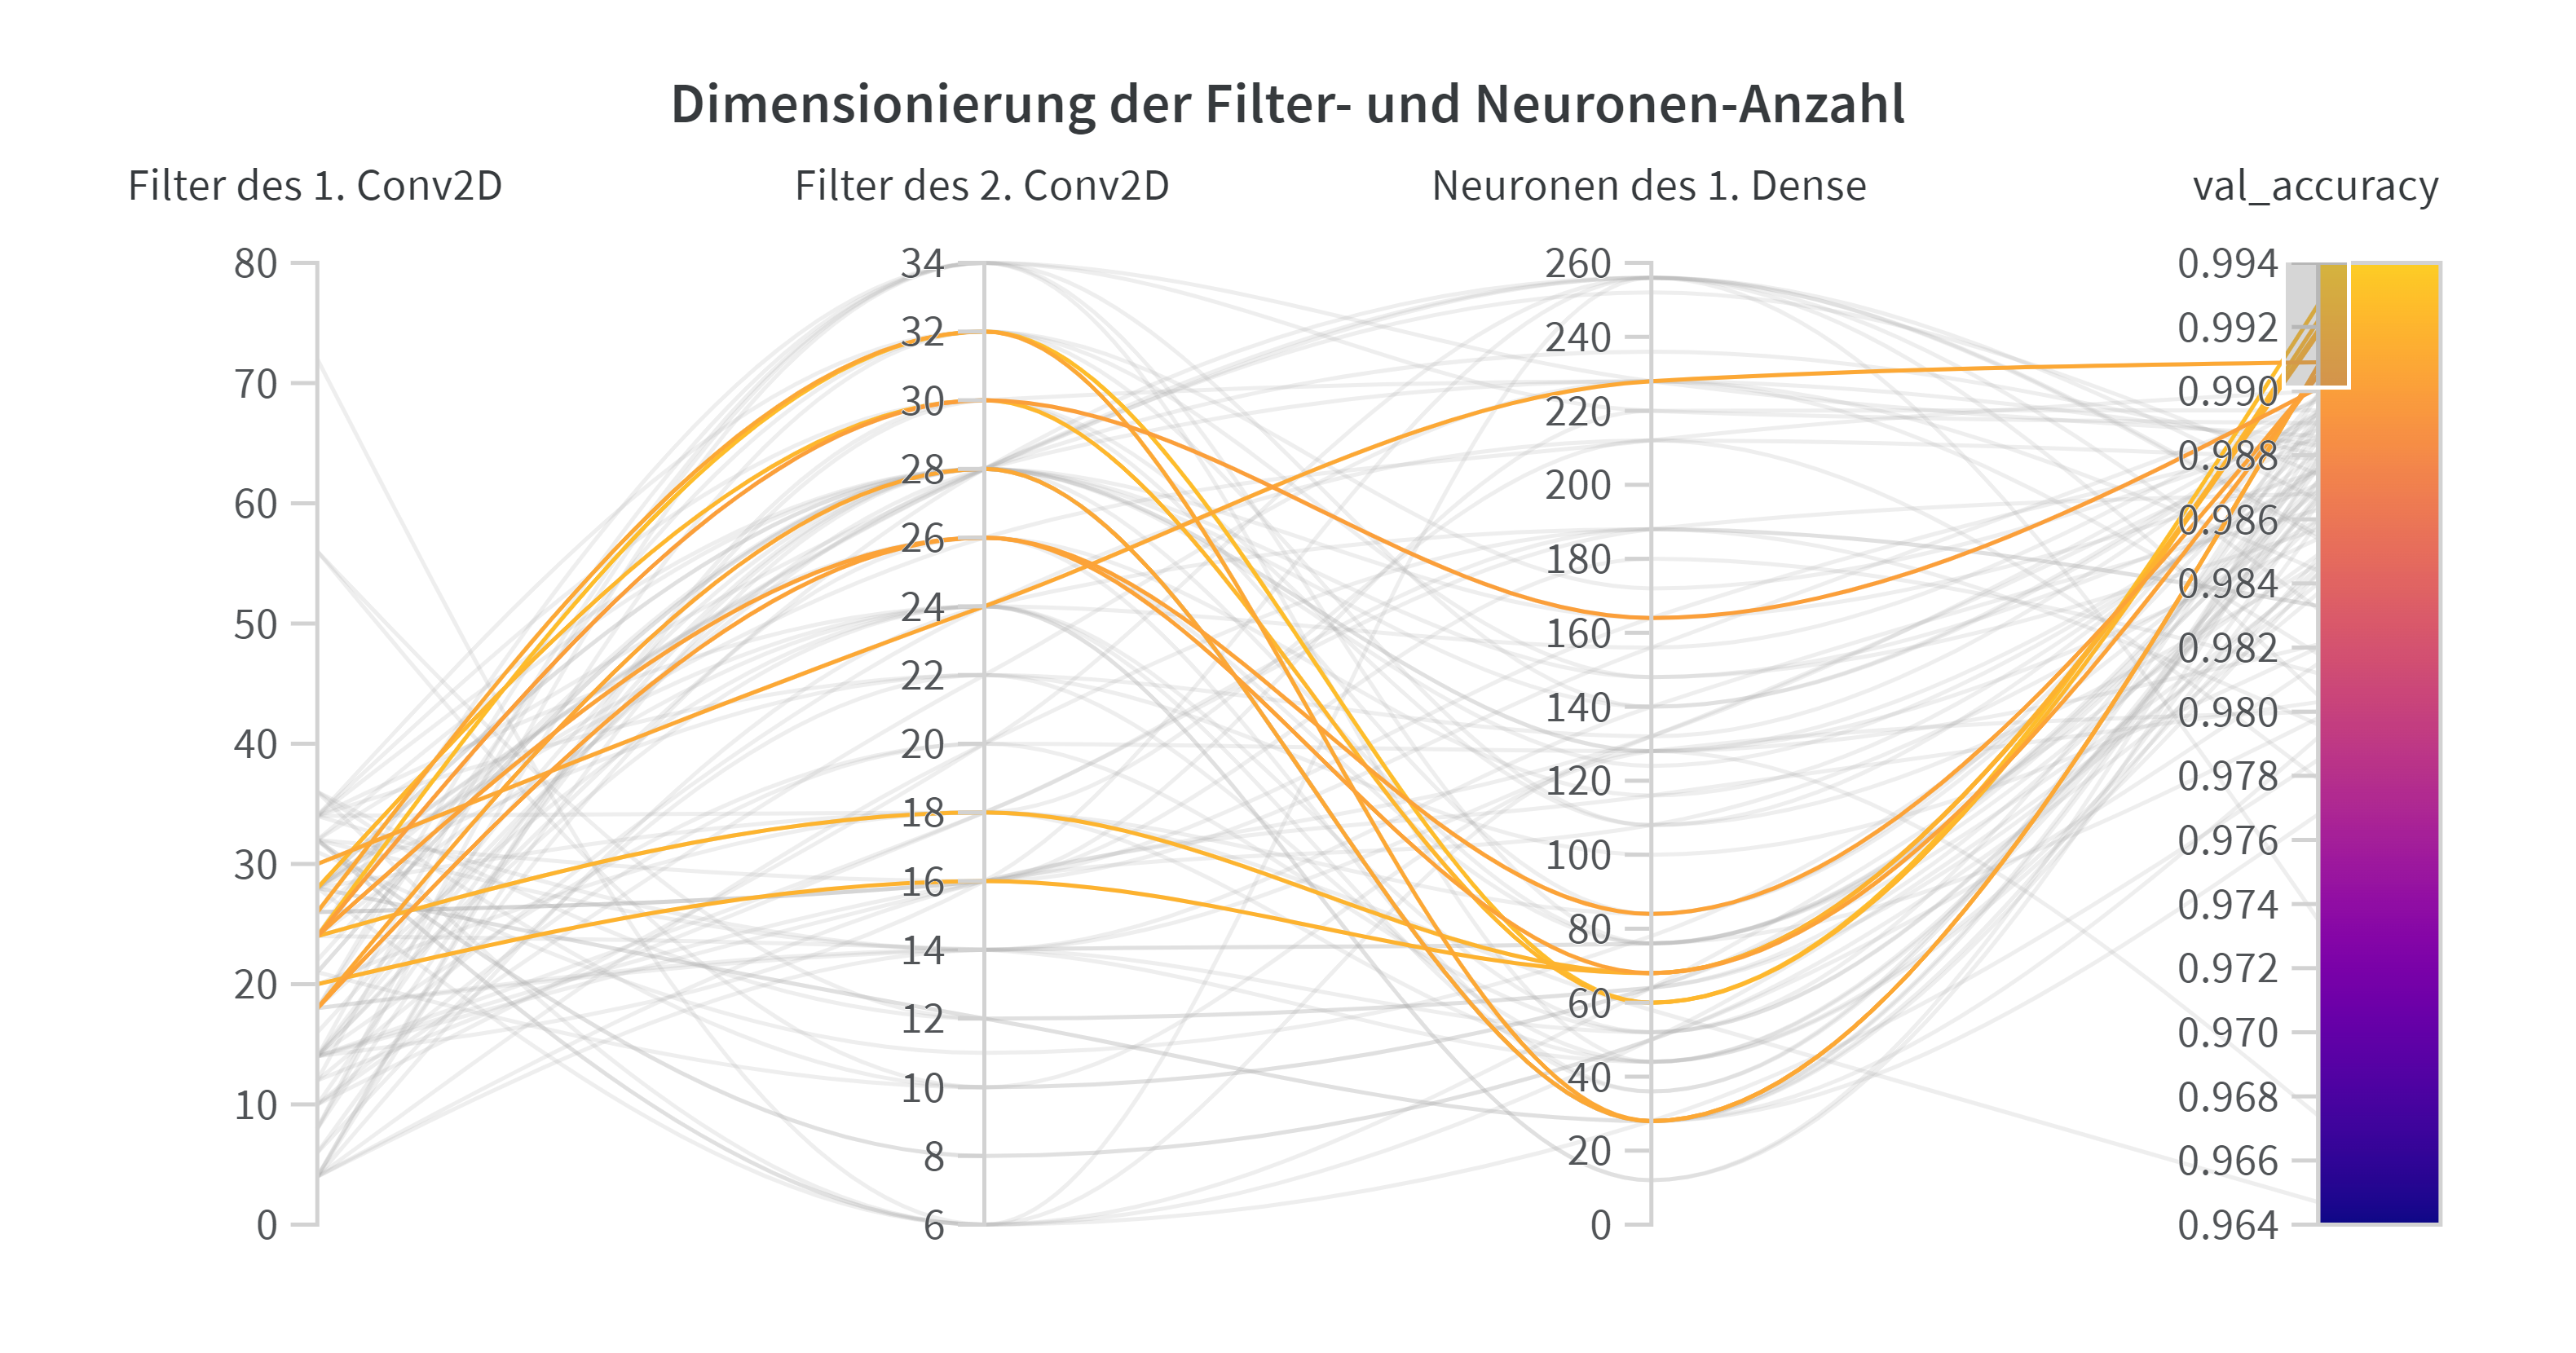
\includegraphics[width=0.7\linewidth]{images/Filter}
	\caption{Etwa 100 Kombinationen aus Filter- und Neuronen-Anzahlen bewertet nach der val\_accuracy. Dokumentiert mit Weight \& Biases}
	\label{fig:filter}
\end{figure}

Zunächst erfolgte die Untersuchung der Filter-Anzahlen in den Convolution-Layern und der Neuronen-Anzahl des ersten Dense-Layer. Das Output-Dense-Layer wird bei 10 Neuronen und der \emph{softmax}-Aktivierungsfunktion belassen, damit jeder Klasse eine Wahrscheinlichkeit zugeordnet wird.\\
Das Raster möglicher Hyperparameter wurde so gewählt, dass (1) eine Abstufung im Convolution-Teil erfolgt, (2) auch Zahlen nicht zur Basis zwei getestet werden und (3) die Parameteranzahl nicht exorbitant groß wird. Das erste Kriterium erwies sich als kontraproduktiv und wird später noch verworfen.\\
Die Ergebnisse von circa 100 Kombinationen sind in \autoref{fig:filter} dargestellt. Hervorgehoben sind die besten Zehn. Die val\_acc ist hoch, für eine Filteranzahl der Convolution-Layers um den Wert 28. Für die Neuronen des ersten Dense-Layers konzentrieren sich der erfolgreichen Kombinationen bei den kleineren Werten. Nach einem weiter eingegrenztem Sweep sind 28 Filter in beiden Convolution-Layern als gewählt und 54 Neuronen für das Dense-Layer. Das Symmetrie-Bedürfnis erkennt Ähnlichkeiten zur Bildgröße von 28x28 Pixeln und wird gleichzeitig enttäuscht, weil 54 weder eine 2er-Potenz noch ein Vielfaches von 28 ist.

\subsection{Wahl der Aktivierungsfunktionen.}

Für die Wahl der Aktivierungsfunktionen wurden ebenfalls Sweeps durchgeführt. Die Ergebnisse sind in \autoref{fig:activ} abgebildet und die besten fünf hervorgehoben. Sie haben die Sigmoid-Funktion im Dense-Layer gemeinsam. Bei den Convolution-Layern zeigte über alle Kombinationen hinweg die Relu-Funktion die stärkste Tendenz zu höher Genauigkeit. Entsprechend wurde gewählt: Relu, Relu, Sigmoid.

\begin{figure}[h]
	\centering
	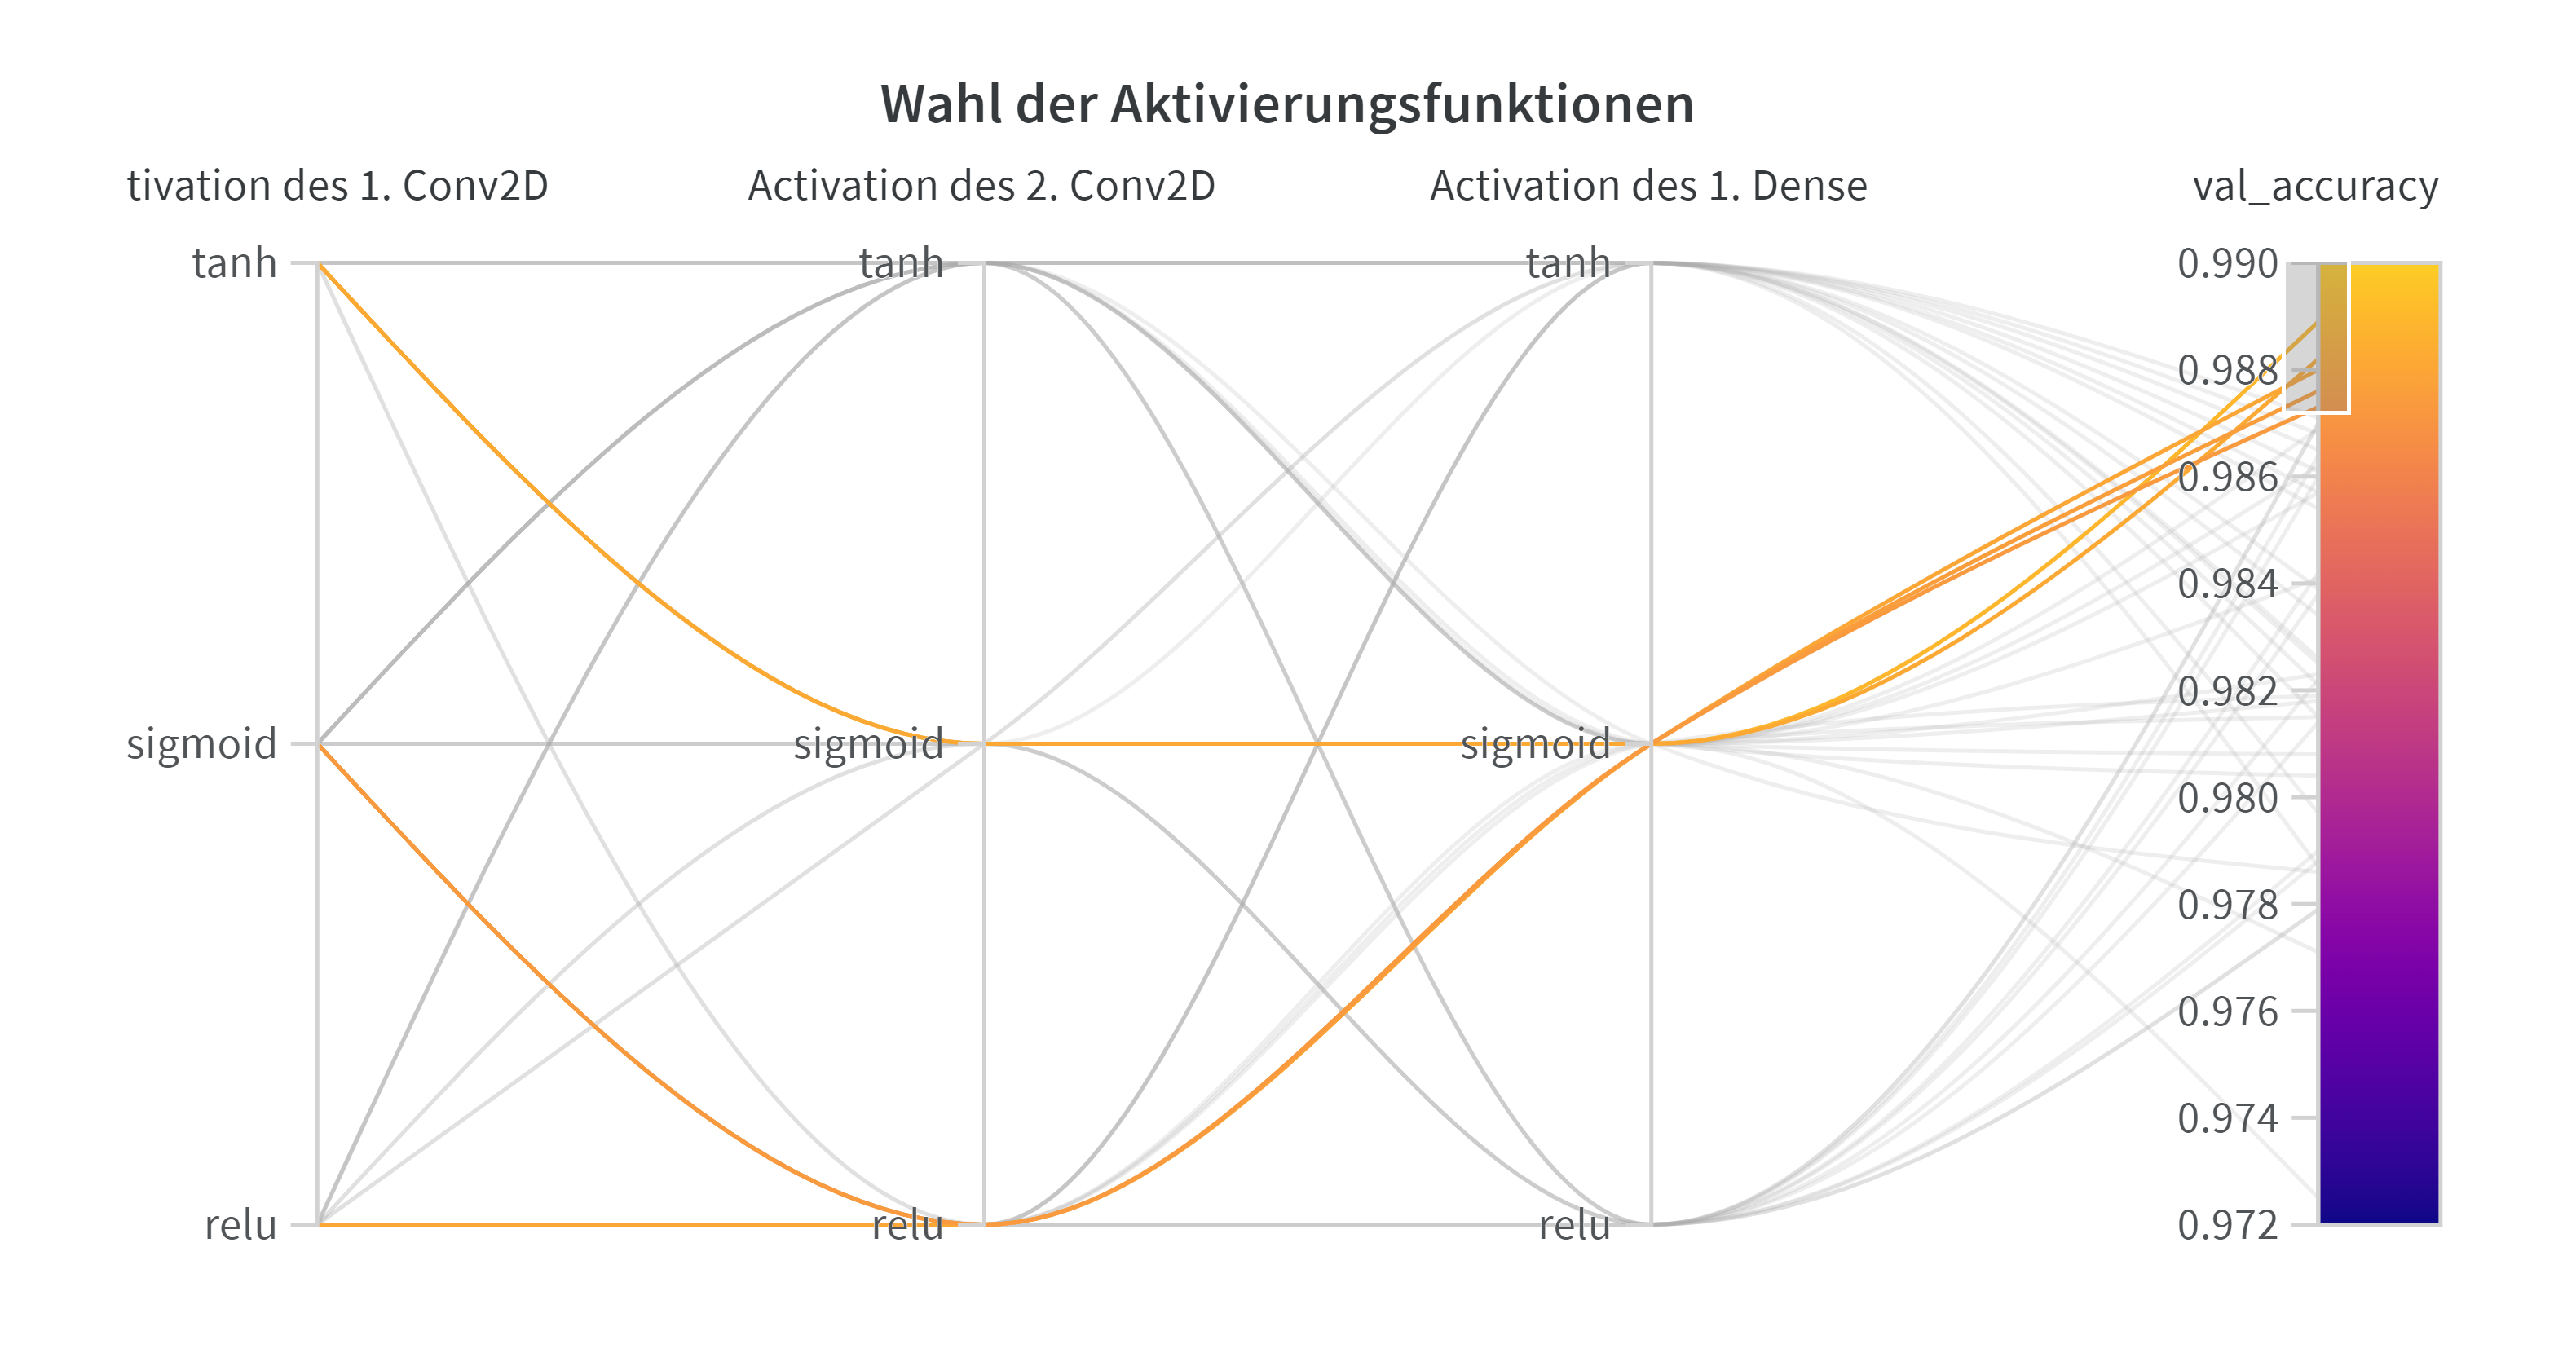
\includegraphics[width=0.7\linewidth]{images/Activ}
	\caption{Kombinationen der Aktivierungsfunktionen bewertet nach der val\_accuracy. Dokumentiert mit Weight \& Biases}
	\label{fig:activ}
\end{figure}

\subsection{BatchNormalization, Dropout und GaussianNoise}

Als drittes wird das Netz zum einen um BatchNormalization vor den MaxPool und Dropout erweitert, weil hiermit konsequent bessere Ergebnisse erzielt wurden.\\
Die Dropout- und GaussianNoise-Werte wurden ebenfalls mittels Weigts \& Biasses getestet. Als erfolgreich Erwiesen sich Dropouts von 0,4 und GaussianNoise von 0.75. \textcolor{red}{papers (dropout gege noverfitting)}. Daraus ergibt sich das in \autoref{wandb} dargestellte Netz mit 95488 Parametern.

\begin{lstlisting} [language=Python, caption=Python-Code, label=wandb]
	tf.keras.layers.InputLayer(input_shape=(28,28,1)),
	tf.keras.layers.Conv2D(filters=28, kernel_size=5, padding='same', activation='relu'),
	tf.keras.layers.BatchNormalization(),
	
	tf.keras.layers.MaxPooling2D(2,2),
	tf.keras.layers.Dropout(0.4),
	
	tf.keras.layers.Conv2D(filters=28, kernel_size=5, padding='same', activation='relu'),
	tf.keras.layers.BatchNormalization(),
	
	tf.keras.layers.MaxPooling2D(2,2),
	tf.keras.layers.Dropout(0.4),
	
	tf.keras.layers.Flatten(),
	
	tf.keras.layers.Dense(54, kernel_regularizer = tf.keras.regularizers.l2(0.07), activation = 'sigmoid'),
	tf.keras.layers.BatchNormalization(),
	
	tf.keras.layers.Dropout(0.4),
	tf.keras.layers.GaussianNoise(0.75),
	
	tf.keras.layers.Dense(10, activation='softmax')
\end{lstlisting}

\subsection{Callbacks - Early Stopping und Variable Learning Rate}

Hinsichtlich des angestrebten Benchmarks sollte die Genauigkeit noch weiter gesteigert werden. Dafür wird der Trainingsprozess mit Callbacks angereichert.\\
Zum einen wird EarlyStopping eingesetzt, um den automatisierten Trainingsprozess zu verkürzen und wenig erfolgreiche Druchläufe abzubrechen. Gleichzeitig werden die besten Ergebnisse gespeichert. 

\begin{lstlisting}[language=Python, caption=Early Stopping, label=er]
	er = tf.keras.callbacks.EarlyStopping(
		 monitor="val_accuracy",
		 patience=10,
	     restore_best_weights=True
	)
\end{lstlisting}

Um darüber hinaus schneller den Grenzwert zu erreichen wird eine Variable Learning Rate verwendet. In Kombination mit dem EarlyStopping zeigte eine gleichmäßige Reduktion mit jeder Epoche besser Ergebnisse, als die Methode ReduceLROnPlateau. In Kombination mit einer Batch Size von 32 ergaben sich die besten Ergebnisse

\begin{lstlisting}[language=Python, caption=Variable Learning-Rate, label=vlr]
	vlr = tf.keras.callbacks.LearningRateScheduler(lambda x: 1e-3 * 0.995 ** x)
\end{lstlisting}

\subsection{Data Augmentation}

Des Weiteren wird die Anzahl an Trainingsdaten mit einer Augmentation erweitert. Dazu kommt der ImageDataGenerator von Keras zum Einsatz. Für Rotation und Zoom werden 0,15 verwendet. Für Shear und Shift 0,1. Die Bilder werden nicht gespiegelt, weil die Zahlen nicht entsprechend symmetrisch sind. Die gewählten Werte haben sich in Weight \& Biases Sweeps als geeignet herausgestellt

\begin{lstlisting}[language=Python, caption=Data Augmentation, label=da]
	
	datagen = tf.keras.preprocessing.image.ImageDataGenerator(
		rotation_range = 15,
		zoom_range = 0.15,
		shear_range = 0.1,
		width_shift_range = 0.1,
		height_shift_range = 0.1,
		rescale = 0,
		fill_mode = 'nearest',
		horizontal_flip=False,
		vertical_flip=False)
	datagen.fit(x_train)

\end{lstlisting}

\subsection{Netzanpassung}

Nachdem die vorausgegangen Methoden wieder stagnierten. Erfolgte eine Anpassung des Netzes.

Zum einen werden zwei aufeinanderfolgende Convolutional Layers mit einer Filtergröße von 3x3 verwendest, anstelle eines mit 5x5. Dadurch ist das Netzwerk in der Lage sein, komplexere und nichtlineare Muster zu erlernen. https://doi.org/10.48550/arXiv.2202.01653 


Strided Convolution für Downsampling: Bei Verwendung einer Convolutional Layer mit Strides von 2 werden die Ausgabefeature-Maps aufgrund des größeren Schrittweitenwerts um den Faktor 2 in jeder Dimension reduziert.
Trainierbare Downsampling-Operation: Im Gegensatz zur Max-Pooling-Schicht, die eine festgelegte Operation (Maximum aus einem Fenster) ohne trainierbare Parameter ist, ermöglicht die Verwendung einer Convolutional Layer mit Strides von 2 das Lernen von Downsampling-Operationen. Die Gewichte in der Convolutional Layer werden während des Trainings angepasst, um die beste Darstellung der Daten zu finden, während gleichzeitig eine Reduzierung der räumlichen Dimensionen erfolgt.

die filter anzah lim 2. conv wurde wie angekündigt erhöhrt auf 56


Zusätzlich wurde auch noch ein Dense layer hinzugefügt mit 82 neuronen (also 28 mehr als das 54 neuronen netzt, für das symmetriebedürfnis)

und nach jedem dropout ein gaussian noise gegen overfitting eingefügt


\section{Zusammenfassunge}

Mit diesen Änderungen wurde bei 50 Netzen...
maximal 99.77 und damit der benchmark


\section{Sonstige Versuche}

Neben dieser ausführlich dokumentierten Optimierung hinsichtlich des Accuracy-Benchmarks wurden an den folgenden Punkte ausprobiert.. 

\subsection{Reduktion der Label}


\begin{lstlisting}[language=Python, caption=Python-Code, label=python_code]
	from scipy.spatial import distance
	
	x_train_best = []  # Array für die ähnlichsten Bilder
	y_train_best = []  # Array für die zugehörigen Labels
	similar_indices = [47647]  # Array für die Indizes der ähnlichsten Bilder
	
	# Berechnung der ähnlichsten Ziffern für jede Klasse von 0 bis 9
	for digit in range(10):
	
	print('Digit:', digit)
	# Filtern der Ziffern nach ihrer Klasse
	class_images = x_train[y_train == digit]
	
	# Berechnung der durchschnittlichen Cosinus-Ähnlichkeit für jede Ziffer zu anderen Ziffern derselben Klasse
	similarities = []
	for i, image in enumerate(class_images):
	avg_similarity = 0
	for other_image in class_images:
	if not np.array_equal(image, other_image):
	# Umwandlung von 28x28 Bildern in Vektoren für Cosinus-Ähnlichkeit
	image_vector = image.flatten()
	other_image_vector = other_image.flatten()
	# Berechnung der Cosinus-Ähnlichkeit
	cosine_similarity = 1 - distance.cosine(image_vector, other_image_vector)
	avg_similarity += cosine_similarity
	avg_similarity /= len(class_images) - 1  # Durchschnittliche Ähnlichkeit zu allen anderen Ziffern der Klasse außer sich selbst
	similarities.append((i, avg_similarity))
	
	# Sortieren nach der durchschnittlichen Ähnlichkeit und Auswahl der ähnlichsten Ziffer
	similarities.sort(key=lambda x: x[1], reverse=True)
	most_similar_index = similarities[0][0]
	
	most_similar_index_train_images = np.where((y_train == digit))[0][most_similar_index]
	most_similar_digit = x_train[most_similar_index_train_images]
	
	print('Index:', most_similar_index_train_images)
	
	# Hinzufügen des ähnlichsten Bildes, seines Labels und seines Index im train_images Array in den Arrays
	x_train_best.append(most_similar_digit)
	y_train_best.append(digit)
	similar_indices.append(most_similar_index_train_images)
	
	# Umwandeln der Listen in numpy arrays
	x_train_best = np.array(x_train_best)
	y_train_best = np.array(y_train_best)
	similar_indices = np.array(similar_indices)
\end{lstlisting}

\subsection{NLP - Tiny Schiller}

tiny schiller referenz

Gandalf in Moria: „Im Zweifelsfall sollte man immer seiner Nase folgen …“




Abschließend ein Zitat des \emph{drunkenSchiller} Models


\end{document}
